\subsection{Trực quan hóa: Số chiều – 3 chiều (3D)}
\textit{3D ThemeRiver} [197] (xem Hình (\ref{fig:f7.15})) là một biến thể 3D của kỹ thuật ThemeRiver [172] (xem Hình 7.16). Phương pháp 3D kế thừa thiết kế hình ảnh cơ bản từ phiên bản 2D của nó: các dữ liệu chuỗi thời gian được thể hiện bằng độ rộng của các dòng có màu sắc khác nhau tạo thành một dòng chảy xuyên suốt theo trục thời gian nằm ngang. Trong biến thể 2D, chỉ có thể biểu diễn một biến dữ liệu trên mỗi dòng, cụ thể là bằng cách thay đổi độ rộng của dòng đó. Giải pháp cải tiến của Imrich cùng cộng sự và các cộng sự sẽ giúp giải quyết hạn chế này. Việc mở rộng thiết kế thêm một chiều thứ ba giúp chúng ta có thể thể hiện thêm được nhiều thông tin trực quan bổ sung: chiều cao (ở dạng 3D) của mỗi dòng có thể được thay đổi để thể hiện thêm những thông tin cần thiết. Thiết kế này đặc biệt phù hợp để hình dung các xu hướng đồng biến bậc ba trong dữ liệu. Imrich và các cộng sự [197] đã tiến hành khảo sát người dùng để đánh giá tính hữu ích của việc biểu diễn 3D này và thực sự đã thu được kết quả tích cực cho thấy biến thể 3D có nhiều ưu điểm hơn so với biến thể 2D. Cụ thể, sự sẵn có của các công cụ tương tác điều hướng 3D thích hợp được nhấn mạnh là một yếu tố quan trọng góp phần vào sự thành công của 3D ThemeRiver.
\begin{figure}[H] % places figure environment here   
    \centering % Centers Graphic
    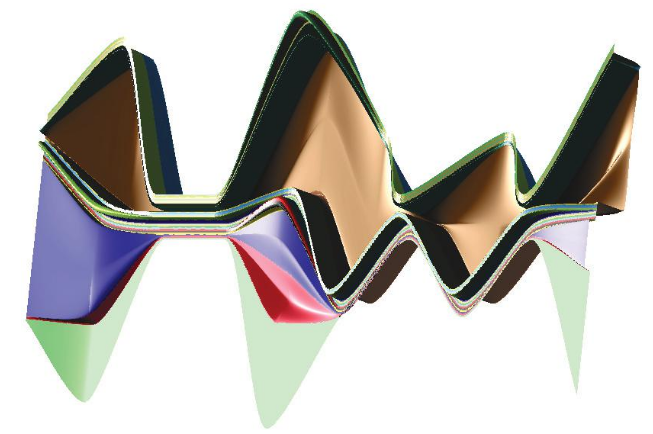
\includegraphics[width=0.8\textwidth]{assets/fig_7_15.png} 
    \caption{3D ThemeRiver [197]. Các dòng có màu riêng biệt tạo thành hình dạng tổng thể của 3D ThemeRiver. Ngoài ra, chiều rộng và chiều cao của các dòng được thay đổi để thể hiện giá trị thay đổi của dữ liệu theo thời gian. Trong hình này, chiều rộng biểu diễn sự phân bố tổng thể của 17 cụm dữ liệu aerosol và chiều cao biểu thị tỷ lệ kẽm. (Được sử dụng với sự cho phép của các tác giả.)} % Creates caption underneath graph
    \label{fig:f7.15}
\end{figure}
Bảng \ref{fig:tb7.16} cung cấp một cách tổng quan về tất cả các kỹ thuật có trong chương này cùng với  các thông tin phân loại chúng. Ta cũng có thể sử dụng bảng này để tìm kiếm các kỹ thuật trực quan hóa đáp ứng các tiêu chí nhất định.
\begin{figure}[H] % places figure environment here   
    \centering % Centers Graphic
    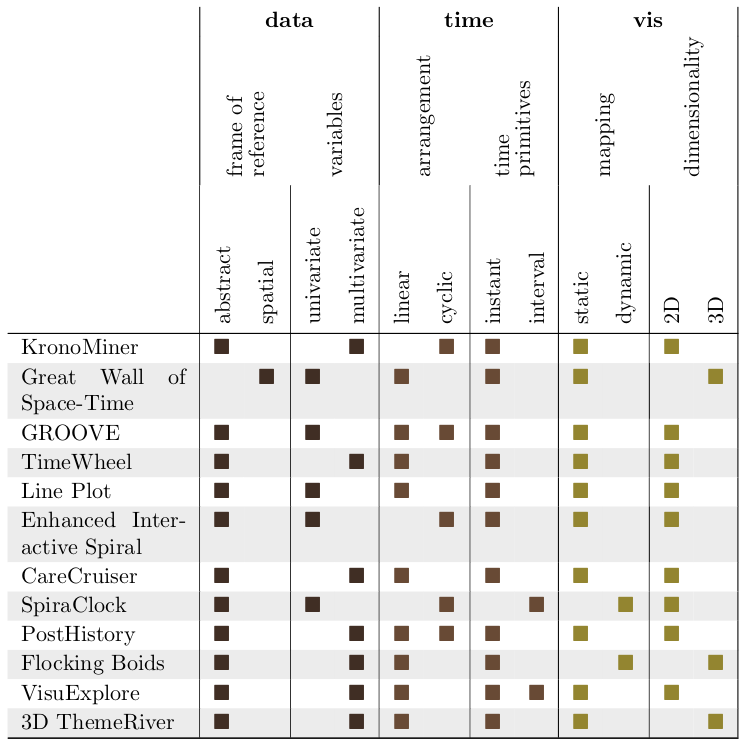
\includegraphics[width=0.9\textwidth]{assets/tb_7_1.png} 
    \caption{Tổng quan và phân loại các kỹ thuật trực quan hóa} % Creates caption underneath graph
    \label{fig:tb7.16}
\end{figure}

